% !TEX root = paper.tex
\iflong
\else
\vspace{-2mm}
\fi
\section{From Single Source to Multiple Sources}

Unfortunately, the analysis for the single source case is not easily extendible to multiple source case. We identify the exact problem here. Consider the case described in Section \ref{subsec:singlecasetwo}. In this case, we show that if $|P'| > |P|$ and $P$ intersects with $P'$, then there is a path available for $P$ (that is $ac \conc
cb' \conc b't$).  We can use this path because it also avoids $e $ (the edge avoided by path $P$). First, we show that the above assertion is not true when we move to multiple source case. Consider the following example (See Figure \ref{fig:multiple}).
Here, $P$ avoids $e$ on $st$ path and $P'$ avoids $e'$ on $s't$ path. $\DET(P)$ starts at $a$ and its intersects $P'$ at $c$. $\DET(P')$ starts at $a'$ and it hits $st$ path at $b'$ and then   passes through $e$. Note that the full path $P$ from $s$ to $t$ is not shown in Figure \ref{fig:multiple}. The reader can check that the  path $ac \conc
cb' \conc b't$ is not an alternate path for $P$ as it passes through $e$. We say that such a path is a bad path because it breaks the easy analysis of single source case (we will formally define bad paths in Section \ref{subsec:pintersects}).
However, we are able to show that the total number of {\em good} paths (paths which are not bad)
is $\ge$ the number of bad paths. Good paths exhibit properties similar to the set
$\RR$ in Section \ref{sec:avoids}. This will help us in bounding them (and thus bad paths too).
%However, we will show that the above bad case does not %happen too often. This completes a short overview of our %approach.
\label{sec:problem}
\iflong

\begin{figure}[hpt!]

\centering
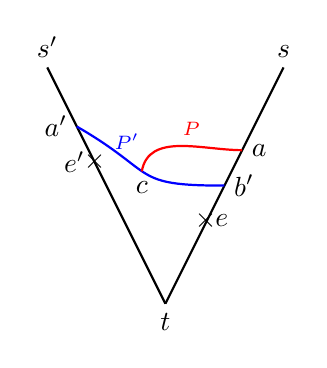
\begin{tikzpicture}[scale=1.5]

\definecolor{dgreen}{rgb}{0.0, 0.5, 0.0}
\begin{scope}[xshift=0cm]
\coordinate (s) at (-1,2);
\coordinate (s1) at (1,2);
\coordinate (t) at (0,0);
\coordinate (ts) at (0,0.4);
\coordinate (b1) at (0.5,1);

\coordinate (a1) at (-0.75,1.5);
\coordinate (a) at (0.65,1.3);
\coordinate (v) at (0.34,0.7);
\coordinate (v1) at (-0.6,1.2);
\coordinate (c) at (-0.2,1.12);

\draw[thick](s)--(t);
\draw[thick](s1)--(t);
\node[above] at (s){$s'$};
\node[above] at (s1){$s$};
\node[below] at (t){$t$};
\node[left] at (a1){$a'$};
\node[right] at (a){$a$};
\node[right] at (b1){$b'$};
\node[below] at (c){$c$};


\draw[blue,thick] (a1) to[out=330,in=180,distance=.8cm]
node[pos=0.3,above]
{\scriptsize  $P'$}  (b1);

\draw[red,thick] (a) to[out=180,in=80]
node[pos=0.4,above]
{\scriptsize  $P$}  (c);

\node at (v1){$\times$};
\node[left] at (v1){$e'$};

\node at (v){$\times$};
\node[right] at (v){$e$};

\end{scope}

\end{tikzpicture}

\caption{The bad case for us: $P' \in (>P)$ intersects with $P$ and then passes through the edge $e$ that $P$ avoids. }
\label{fig:multiple}
\end{figure}

\fi
Once again we will fix a vertex $t$ and show that  the number of replacement paths from
$s \in S$ to $t$ that also avoids $t_s$ is $ O(\sqrt {\sigma n})$.
Let $\BFS(t)$ denote  the  union of all  shortest paths from $t$ to $s \in S$.
The reader can check that the union of these paths does not admit a cycle, so we
can assume that its a tree rooted at $t$. Since $\BFS(t)$ has at most $\sigma$
leaves, the number of vertices with degree $> 2$ in $\BFS(t)$ is $O(\sigma)$.
We now contract all the vertices of degree 2 (except $t$ and $s \in S$) in $\BFS(t)$
to get a tree that only contains
leaves of $\BFS(t)$, the root $t$, all the sources and all other vertices
with degree $> 2$ in $\BFS(t)$.
\begin{definition} (\SBFS($t$))
\SBFS($t$) is a tree obtained by contracting all the vertices with degree exactly 2 in $\BFS(t)$
except $t$ and source $s \in S$.
\end{definition}

\begin{definition} (Intersection vertex and segment in \SBFS($t$))

\noindent Each node  \SBFS$(t)$  is called an intersection vertex.
An edge $xy \in$ \SBFS($t$) denotes a path between two vertices in $\BFS(t)$.
We call such an edge in \SBFS\  a segment. We use this term in order to differentiate between  edges in $\BFS(t)$ and  \SBFS($t$).
Also, we will use the following convention: if $xy$ is a segment,
then $y$ is closer to $t$ than $x$.
\end{definition}
\noindent \SBFS($t$) has at most $\sigma$
vertices with degree $\le 2$. This implies that there are at most $O(\sigma)$
intersection vertices and segments in \SBFS($t$).
%Similarly, the total number of
%segments in \SBFS($t$) is $O(\sigma)$.

As in the single source case, we would like to find the preferred path for each avoided edge on the $st$
path where $s \in S$. However, we don't have enough space to store all these paths.
Also storing all  paths seems wasteful.
Consider two preferred replacement paths $P$ and $P'$ that start from $s$ and $s'$ respectively.
These two paths meet at an intersection vertex $x$ after which they are same, that is, they take
the same detour to reach $t$. Storing both $P$ and $P'$ seems wasteful as they are essentially
the same path once they hit $x$.  To this end, we only store preferred path
corresponding to each segment in \SBFS($t$). We now describe our approach in detail.

Let $xy$ be a segment in \SBFS($t$). We divide replacement paths whose detour start in $xy$ into
two types:
\begin{itemize}[noitemsep,nolistsep]
  % \item[($\TZE$)] Replacement path whose failed vertex %is  an intersection vertex in \SBFS(t).

%   Thus for the next two sets, the failed vertex is not %an intersection vertex in \SBFS(t).
   \item[] $\TON(xy)$: Preferred replacement paths from $x$ to $t$ whose detour starts in $xy$
    but the avoided edge lies in $yt_x$.

   \item[] $\TTW(xy)$: Preferred replacement paths from $x$ to $t$ whose
   start of detour and avoided edge both lie strictly inside segment $xy$ (that is, detour cannot
   start from $x$ or $y$).
\end{itemize}


\noindent Let $\TON := \cup_{xy \in \text{\SBFS($t$)}} \TON(xy)$ and
$\TTW := \cup_{xy \in \text{\SBFS($t$)}} \TTW(xy)$. The set  $\TON$ helps us to weed out
simple preferred replacement paths.
We will show that we can store  preferred replacement paths in  $\TON$ in
$O(\sigma)$ space --  one per segment in \SBFS($t$).
The hardest case for us in $\TTW$, which contains bad paths.
%$\TON$ helps us weed out simple replacement paths so that we don't have
%to bother about them when we are analyzing the harder case,
%that is paths in $\TTW$.
%For $\TTW$, we have to take care of the bad paths.
Let $\BP$ denote the set of bad paths in $\TTW$. We will show  that
$|\BP| \le |\TTW \setminus \BP|$ (the number of bad paths is $\le$ number of good paths in $\TTW$)
and $|\TTW \setminus \BP| =  O(\sqrt{n\sigma})$ (the number of good path is $ O(\sqrt{n\sigma}$)).
This implies that $|\TTW| =  O(\sqrt{n \sigma})$. %This would imply that
%the total number of path from $s \in S$ to $t$ that don't %pass through
%$t_s$ is $\tilde O(\sqrt{n \sigma})$.

Since $\TON$ and $\TTW$ are of size $O(\sqrt{n\sigma})$, we can make a data-structure
of size $O(\sqrt{n\sigma})$.
In this data-structure, we have stored a preferred path for each segment.
However, we have to answer queries of type $\textsc{Q}(s,t,e)$
where $s$ is a source.
%It is not clear how to use our data-structure
%to answer this query correctly.
In Section \ref{sec:data}, we will see
how to use preferred paths of segments to
answer queries in $\tilde O(1)$ time.
